\section{PGAS and OP2}

This section outlines the designs for our PGAS memory backend for OP2. To do this, it begins by introducing the primary assumptions/constraints that underpin the designs. Then, it will introduce the current MPI setup, finally followed by the two designs
and their likely risks/effects. To conclude it will cover how we intend to move further with the project from this point.

\subsection{Application Level Considerations}
The following considerations regard how applications function in a HPC environment. This is particularly important given impact each of these may have on performance. 

There are two key points that cover the majority of performance considerations. They are most broadly `scaling' and `caching'. Scaling refers to the effects of strong or weak scaling on the application, with particular effects on the relationship between network and compute time. Whereas, caching encompasses the effects of memory access patterns, memory access times, cache temperature, and finally cache size. All of the given caching points are highly interdependent but are given separately for clarity and comprehensiveness.

\subsubsection{Scaling}
Scaling can be either strong or weak. Strong scaling refers to the scaling of performance with a variable number of worker processes on a statically sized global problem, whereas weak scaling maintains a static amount of work per process for a variable number of processes (i.e. the problem size is a function of the process count). The majority of applications using OP2 will exhibit strong scaling. This strong scaling will change the relative sizes of the halo elements to the core elements and thus affect the network compute relationships. As previously stated, minimising the sizes of the halos is paramount to performance, hence the efforts of the optimal partitioning libraries. 

With this information, it is important to consider the effects of adding local workload to improve network efficiency. It is a fluid and complex balancing act to find an effective compromise between network and compute overheads for variable problem sizes and process counts.

\subsubsection{Caching}

%do this somewhere else??
Caching is a method of storing frequently accessed data in small, very fast, memory banks close inside (or very close to) the CPU. In modern day CPUs this involves a hierarchy moving from very small and very fast, to relatively large and slow - though is still order of magnitudes faster than main memory (RAM). The fastest level (L1) is often local to each core, L2 is often shared between 2 or more cores, with the slowest (L3) shared between all cores. Importantly, each level of the hierarchy contains a copy of all information stored in the previous levels. This is to help improve cache miss performance.

The current MPI design is built to optimise cache hit rates. For example, OP2 currently employs an Array of Structs (AoS) memory layout to improve caching in this hierarchical environment. Each struct is likely to fit into a minimal number of cache lines such that they can all move up and down the hierarchy together - a very efficient design in this context.  Importantly, AoS is often very slow in other environments, with a Struct of Arrays enabling pre-fetcher and SIMD\footnote{Single Instruction Multiple Data} operations. Clearly, performance is highly context dependant so care must be taken to make informed decisions.

%find somewhere to cite that might back this up.
Thus it is critical for the GPI design to be similarly built around these considerations, especially as memory is often the primary bottleneck in HPC environments. 

\subsection{GASPI Constraints}

% Reminders of the constraints given GASPI.
As individual segments have to be contiguous in memory, an important consideration is the maximum size they can be. If a segment is too large, either the OS memory allocation could fail (although this will be system dependent) or GASPI may decline it based on system capabilities including those of the network interface card (NIC). This has been vaguely warned against in the GASPI specification, stating ``hardware limitations'' and ``performance penalties'' regarding allocating large segments.  This is likely because, the NIC must store basic data structures enabling naive page swap functionality without CPU interference. Should this data structure be small, it will limit the total mapped memory region the NIC can support without CPU interference, causing potentially significant performance penalties. 

%be able to handle a page swap of a certain size during RDMA, therefore more pages mean more swaps, reducing overall performance. These factors all require that the segment sizes should be minimal.

Following from this, the GASPI 17.1 specification also warns about the performance impact of having a large number of segments. This is not a major concern for most applications, but it does limit the scalability of a solution where the number of segments scales with the problem size (e.g. one segment per \texttt{op\_dat}). 

This vagueness in the specification causes significant problems for system designers. There exists no concrete definition as to what is `too large' or `too many', nor any method given to use hardware information to estimate these values - everything must be evaluated experimentally. 

It should be noted that when working with GASPI-MPI interoperability, overlapping MPI and GASPI communication results in undefined behaviour and so should be avoided. Even if there are no immediate problems, there are no assurances that this will always be the case.

Finally, the GASPI specification is very lean and thus only provides only a minimal set of functions for communication and synchronisation. Therefore, for more complicated operations, they require bespoke implementations. This includes things like safety wrappers to ensure communication correctness as well as the allgather function. 


\subsection{OP2 Integration}

Not only must these designs be performant and provide an effective alternative to the MPI backend, it they must also not prohibit other configurations such as CUDA, OpenMP or codegeneration.  

%TODO Say something about the makefiles, and ensuring we make all the same assumptions as the MPI one. 


\subsection{GASPI For OP2}

% Overview of how memory setup currently works in OP2 and the problems this causes to us. 
Currently, all \texttt{op\_dat} data is non-contiguous (at the dat level), in other words, all primary data is part of an Array of Structs (AoS) where \texttt{op\_dat} structs are contained in an \texttt{op\_dat\_list} and each \texttt{op\_dat} points to an arbitrary memory location that stores the actual data. The structure of \texttt{op\_dat->data} can be seen in figure \ref{fig:Halo_set_example_table}. The reason for an AoS setup is firstly to enable greater use of cache lines and modern cache hierarchies to improve hit rates. Secondly, it is to ensure coalescence of data for easier and more efficient data exchange with GPU memory or the network. % TODO: I haven't double checked this against the original dev doc yet

This AoS setup is suitable for the MPI API as each node has full control over where it can read/write to/from locally, they can be any arbitrary memory address. This extent of control is not available in GPI. GPI requires the creations of segments (due to RMA/RDMA pinning RAM pages for the NIC), of which there cannot be an excessive number of due to "hardware limitations" and "performance penalties" as previously mentioned. Therefore, sparsely located data, as seen in OP2 does not lend itself well towards GASPI segments. However, in the case of export sets, the data must be packed and copied into a buffer region before the asynchronous send (due to data dependencies and enabling the overlap of communication and computation). This buffer region can be a single homogeneous segment - well suited to GPI. Unfortunately for import sets this is not the same. The current MPI implementation is able to receive the imported data elements directly into the import section of the \texttt{op\_dat->data} array, thus when the receive is finished, the data is fully ready to continue with computation. The layout for this can be seen in figure \ref{fig:op_set_layout}. However, for GPI all data transfer must occur between segments; the benefits and drawbacks to the options in handling this limitation are presented below.
\begin{figure*}
    \centering
    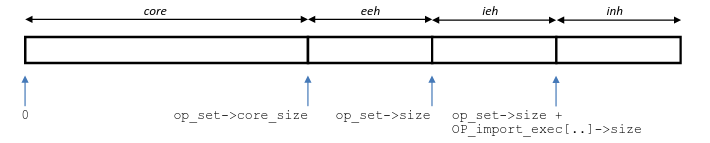
\includegraphics[width=\linewidth]{figures/op_mpi_set_diagram.png}
    \caption{Element order of \texttt{op\_set} after halo creation}
    \label{fig:op_set_layout}
\end{figure*}